\documentclass[conference,spanish]{IEEEtran}

% ── Codificación y Lengua ──────────────────────────────────────────────────────
\usepackage[utf8]{inputenc}
\usepackage[T1]{fontenc}
\usepackage[spanish,es-noshorthands,es-tabla]{babel}

% ── Matemáticas ───────────────────────────────────────────────────────────────
\usepackage{amsmath, amssymb}

% ── Imágenes y diagramas ──────────────────────────────────────────────────────
\usepackage{graphicx}
\usepackage{float}
\usepackage{tikz}
\usetikzlibrary{positioning,arrows.meta}

% ── Tablas ────────────────────────────────────────────────────────────────────
\usepackage{booktabs}
\usepackage{array}

% ── Hipervínculos ─────────────────────────────────────────────────────────────
\usepackage[colorlinks=true, linkcolor=blue, urlcolor=blue, citecolor=blue]{hyperref}

% ── Otros ─────────────────────────────────────────────────────────────────────
\usepackage{microtype}
\usepackage{cite}

% ═══════════════════════════════════════════════════════════════════════════════
\begin{document}

\title{Predicción del Retraso al Final de una Ruta de Bus Urbano en Cusco con Datos de Control de Horarios, GPS y Aprendizaje Automático\\
\large Paper final --- Aprendizaje de Máquina, PUCP 2026-2}

\author{
    \IEEEauthorblockN{
        Claudia Serpa,\;
        Nicoll Tone,\;
        Reynaldo Mamani,\;
        Jeremy Aldama
    }
    \IEEEauthorblockA{
        Facultad de Ciencias e Ingeniería,
        Pontificia Universidad Católica del Perú, Lima, Perú
    }
}

\maketitle

% ── Resumen ───────────────────────────────────────────────────────────────────
\begin{abstract}
Se predice, cuando un bus pasa por el punto de control 10 de 18 de una ruta de Cusco, cuántos minutos llegará tarde o temprano al último punto de control, y se traduce esa predicción en tres clases operativas. Se usan los dos archivos del sistema de transporte inteligente de la ciudad: el registro de control de horarios (4\,707 vueltas de 45 buses, 6 de enero--1 de febrero de 2025) y 1,63 millones de posiciones GPS. Tras una limpieza documentada quedan 4\,559 vueltas, 4\,004 con el último punto observado. Además de los retrasos ya observados, la hora y el día, se construyen variables en tiempo real del tramo que el bus aún no recorre: el retraso que ganaron entre los puntos 10 y 14 las vueltas que pasaron por ahí en los 30 min previos y la velocidad GPS de los buses que van adelante. Se comparan tres líneas base con Ridge, Random Forest y HistGradientBoosting mediante validación cruzada \textit{forward-chaining} por días, y la prueba (27 de enero--1 de febrero) se evalúa una sola vez por modelo. HistGradientBoosting obtiene un MAE de 2,76 min (IC 95\,\% por día: 2,28--3,34), un 36\,\% menos que la persistencia (4,32 min), y $R^2=0{,}76$ (0,62--0,84). Las variables en tiempo real bajan el MAE de validación cruzada de los tres modelos, pero en la prueba HistGB queda igual que sin ellas (diferencia de 0,01 min, IC $-0{,}06$--0,11); sí bajan el error del sábado (de 4,61 a 4,30 min). Para el despachador, clasificar la vuelta en adelantada, puntual o retrasada con la predicción de HistGB logra un F1 macro de 0,70 (0,62--0,77), frente a 0,50 de la persistencia, y casi nunca confunde una vuelta retrasada con una adelantada. El agrupamiento de los perfiles de 18 retrasos separa vueltas de madrugada que llegan adelantadas y un grupo de retraso alto, compuesto en un 72\,\% por sábados, donde se concentra el error. La meta de $R^2\ge0{,}80$ no se demuestra desde el punto 10; en validación cruzada se alcanza desde el punto 14. Se entrega una demo interactiva que recorre las vueltas reales de la prueba.
\end{abstract}

\begin{IEEEkeywords}
transporte público, AVL, GPS, predicción de retrasos, puntualidad, gradient boosting, agrupamiento, validación temporal, Cusco
\end{IEEEkeywords}

% ═══════════════════════════════════════════════════════════════════════════════
\section{Introducción}

En el transporte urbano de Cusco, la puntualidad respecto al horario programado es la principal medida de calidad que perciben los usuarios y que controlan los operadores. Las empresas ya registran, para cada vuelta, la hora programada y la hora real de paso por puntos de control, y monitorean la posición GPS de cada bus. Sin embargo, esa información se usa hoy para registrar o sancionar el retraso una vez ocurrido, no para anticiparlo.

Los datos muestran que el problema es real y crece a lo largo de la ruta. En los primeros puntos de control el retraso mediano es 0 o $-1$ min, pero desde el punto 14 la mediana sube a 1--3 min y el cuartil superior llega a 6--7 min. En el último punto, el 38\,\% de las vueltas llega más de 3 min tarde y el 17\,\% llega 2 min o más adelantada.

\textbf{Problema.} Sea $d_{\ell,k}=t^{\mathrm{real}}_{\ell,k}-t^{\mathrm{prog}}_{\ell,k}$ el retraso de la vuelta $\ell$ en el punto de control $k$ (positivo si el bus va tarde). Cuando el bus pasa por $k$, se busca
\begin{equation}
\hat d_{\ell,18}=f_\theta\!\left(\mathbf x_{\ell,\le k}\right),
\end{equation}
donde $\mathbf x_{\ell,\le k}$ contiene únicamente información disponible en ese instante: los retrasos observados hasta $k$, el horario, el calendario, el vehículo y el estado reciente de los tramos siguientes según otras vueltas y el GPS. El experimento principal fija $k=10$, a mitad de la ruta, con 8 puntos por recorrer. La hora de llegada estimada es $\hat t^{\mathrm{real}}_{\ell,18}=t^{\mathrm{prog}}_{\ell,18}+\hat d_{\ell,18}$, la misma formulación residual sobre una referencia que usan trabajos recientes \cite{li2024arrivalnet,hu2022deepreta}. Para la operación, la predicción se convierte además en una clase (adelantada, puntual o retrasada).

\textbf{Por qué es un problema de aprendizaje automático.} El retraso depende de forma no lineal de la hora, el día, el horario programado y la propagación del retraso previo. La regla ``el retraso actual se mantiene'' es una línea base razonable, pero deja mucho error sin explicar (Sección~\ref{sec:resultados}).

\textbf{Contribuciones.} (i) Reglas de limpieza cuantificadas para el registro de horarios, incluida la corrección de una interpretación errónea de la propuesta. (ii) Una comparación de modelos con validación temporal por días y una prueba evaluada una sola vez, con intervalos de confianza por día. (iii) Variables en tiempo real del tramo siguiente, construidas sin fuga de información a partir de otras vueltas y del GPS. (iv) Una clasificación de puntualidad útil para el despachador, un agrupamiento de perfiles de retraso que explica dónde falla el modelo y una demo interactiva.

\textbf{Organización.} La Sección~II presenta los objetivos; la III, los trabajos relacionados; la IV, los datos; la V, la metodología; la VI, los resultados; la VII, la demo; la VIII, la discusión; la IX, las conclusiones; y la X, el entorno para reproducir los experimentos.

% ═══════════════════════════════════════════════════════════════════════════════
\section{Objetivos}

\textbf{Objetivo general.} Desarrollar y comparar modelos de aprendizaje automático que anticipen el retraso de un bus en el último punto de control de su vuelta, a partir de los datos del sistema de transporte inteligente de Cusco, con un error menor que el de las líneas base operativas.

\textbf{Objetivos específicos.}
\begin{enumerate}
    \item Limpiar el registro de horarios con reglas explícitas y cuantificadas, y caracterizar sus problemas de calidad.
    \item Comparar Ridge, Random Forest y HistGradientBoosting contra tres líneas base con validación temporal sin fuga de información.
    \item Medir cuánto aportan las variables en tiempo real derivadas de otras vueltas y del GPS.
    \item Medir el error según el punto de control desde el que se predice, con hiperparámetros ajustados para cada punto.
    \item Clasificar la puntualidad de la vuelta y agrupar los perfiles de retraso.
    \item Construir una demo interactiva que muestre el funcionamiento de la solución.
\end{enumerate}

\textbf{Metas fijadas antes de evaluar la prueba.} (i) Superar a la mejor línea base en MAE. (ii) Alcanzar $R^2\ge0{,}80$, que responde a la indicación del docente de fijar un umbral de desempeño del 80\,\%. Como el enunciado no especifica la métrica, se eligió $R^2$ porque es la proporción propia de la regresión. Tiene una limitación: depende de la varianza del objetivo en el conjunto evaluado (Sección~\ref{sec:desglose}). Por eso la métrica principal es el MAE en minutos, y el $R^2$ se usa solo para contrastar la meta.

% ═══════════════════════════════════════════════════════════════════════════════
\section{Trabajos Relacionados}

La predicción del tiempo de llegada y del retraso de buses es un tema amplio. La revisión de Reich et al.\ \cite{reich2019} concluye que ninguna familia de métodos domina en todos los contextos y que los resultados son poco comparables entre estudios; la de Kumar et al.\ \cite{kumar2025review} organiza los enfoques en ingenuos, basados en física y guiados por datos. Ello justifica comparar varios modelos bajo un mismo diseño experimental. La Tabla~\ref{tab:sota} resume los trabajos más cercanos.

\textbf{Primeros enfoques.} Chien et al.\ \cite{chien2002} y Jeong y Rilett \cite{jeong2004} usaron redes neuronales con datos AVL y superaron a los modelos históricos y de regresión. Yu et al.\ \cite{yu2006} aplicaron máquinas de vectores de soporte con variables de segmento, hora y tiempo de recorrido previo, y en paraderos con varias rutas SVM superó a redes neuronales, $k$-NN y regresión lineal \cite{yu2011}. Achar et al.\ \cite{achar2020} propusieron un filtro de Kalman espacial que aprende correlaciones entre tramos: el estado de un tramo informa sobre el siguiente, la misma idea que motiva nuestras variables en tiempo real.

\textbf{Ensambles de árboles e interpretabilidad.} Martyanov et al.\ \cite{martyanov2026} es el trabajo más cercano a nuestra formulación: definen el retraso como la diferencia entre la llegada observada y la programada en cada parada, comparan Random Forest, XGBoost y CatBoost con validación cruzada temporal anidada y usan SHAP. Obtienen MAE $\approx$ 3,6 min y $R^2\approx$ 0,44, y encuentran que la hora del día y la posición en la ruta son las variables más influyentes.

\textbf{Aprendizaje profundo.} Petersen et al.\ \cite{petersen2019} emplearon una ConvLSTM multisalida sobre 1,2 millones de observaciones de una línea de Copenhague y redujeron el MAE de 3,23 min (media histórica) a 1,99 min. Boudabbous et al.\ \cite{boudabbous2026} predicen retrasos en toda la red de Montreal con LSTM, XGBoost y transformers bajo validación \textit{walk-forward}, y usan PCA para comprimir 1\,683 variables. En datos tabulares, los modelos de árboles suelen igualar o superar a las redes profundas \cite{grinsztajn2022}; con unas 4\,000 vueltas, se priorizaron los ensambles.

\textbf{Otros medios y escala industrial.} DeeprETA de Uber \cite{hu2022deepreta} predice el residuo entre la estimación del motor de rutas y la llegada observada, y el sistema Wide-Deep-Recurrent de DiDi \cite{wang2018wdr} corrige estimaciones base con un modelo aprendido. Ambos respaldan modelar la desviación respecto a una referencia (aquí, el horario).

\textbf{Enfoques no supervisados.} Degeler et al.\ \cite{degeler2021} agrupan con $k$-means estados de operación (normal, retrasado, apelotonamiento) a partir de AVL y eligen $k$ con el coeficiente de silueta. En Cusco, Rojas-Bustamante et al.\ \cite{rojas2023} usaron aprendizaje no supervisado sobre trazas GPS de transporte público para perfilar la accesibilidad a servicios.

\textbf{Antecedentes en Perú.} Un trabajo con datos de Cusco \cite{cusco2024} aplica LSTM y ConvLSTM a 1,6 millones de registros GPS de buses y reporta un MAE de 19,55 s, pero predice tiempos de viaje, no el retraso respecto al horario. En Lima, Traverso et al.\ \cite{traverso2025} entrenaron Random Forest con registros del Corredor Metropolitano y reportan $R^2=0{,}9998$; valores tan altos, junto con una partición 70/30 sin descripción temporal, motivan cautela y subrayan la necesidad de evitar la fuga de información \cite{kaufman2012}.

\textbf{Evaluación y umbrales.} En series temporales, la validación cruzada aleatoria puede inflar el desempeño \cite{bergmeir2012}; por ello se usa partición cronológica. En puntualidad de buses, una convención muy extendida considera a tiempo una llegada con hasta 1 min de adelanto y 5 min de retraso \cite{tcrp2003}; nuestras clases la adoptan.

\textbf{Brecha que se aborda.} No se encontraron trabajos que predigan el retraso en puntos de control de rutas de Cusco, una ciudad con topografía y operación (puntos con horario fijo y sanciones por adelanto) distintas a las estudiadas, ni que combinen el registro de horarios con el GPS de los buses precedentes.

\begin{table*}[t]
\centering
\caption{Resumen de trabajos relacionados}
\label{tab:sota}
\footnotesize
\begin{tabular}{@{}p{3.4cm}p{4.3cm}p{4.0cm}p{4.9cm}@{}}
\toprule
\textbf{Trabajo} & \textbf{Datos} & \textbf{Modelos} & \textbf{Resultado clave}\\
\midrule
Yu \textit{et al.} 2006, 2011 \cite{yu2006,yu2011} & AVL; paraderos con varias rutas & SVM, ANN, $k$-NN, regresión lineal & SVM obtiene los mejores resultados\\
Achar \textit{et al.} 2020 \cite{achar2020} & GPS de buses, tráfico heterogéneo & Filtro de Kalman espacial & Captura correlaciones espacio-temporales por tramo\\
Petersen \textit{et al.} 2019 \cite{petersen2019} & Línea de Copenhague; 1,2 M obs. & ConvLSTM, LSTM, media histórica & MAE 1,99 min frente a 3,23 min (media histórica)\\
Martyanov \textit{et al.} 2026 \cite{martyanov2026} & AVL de Varsovia (retraso por parada) & RF, XGBoost, CatBoost + SHAP & MAE $\approx$ 3,6 min; RMSE $\approx$ 5,4 min; $R^2\approx$ 0,44\\
Boudabbous \textit{et al.} 2026 \cite{boudabbous2026} & Red de Montreal; seis meses & LSTM, XGBoost, xLSTM, transformers; PCA & LSTM compacta: mejor compromiso precisión--eficiencia\\
Degeler \textit{et al.} 2021 \cite{degeler2021} & AVL, apelotonamiento & $k$-means (silueta) & Estados: normal, retrasado, apelotonado\\
Trabajo en Cusco \cite{cusco2024} & 1,6 M registros GPS, Cusco & LSTM, ConvLSTM & MAE 19,55 s (tiempo de viaje)\\
Traverso \textit{et al.} 2025 \cite{traverso2025} & Corredor Metropolitano, Lima & Random Forest & $R^2=0{,}9998$ (requiere cautela)\\
Hu \textit{et al.} 2022 \cite{hu2022deepreta} & ETA global de Uber & Transformer lineal residual & En producción; modela el residuo de la ETA base\\
\bottomrule
\end{tabular}
\end{table*}

% ═══════════════════════════════════════════════════════════════════════════════
\section{Conjunto de Datos}

Los dos archivos describen una sola ruta circular de 18 puntos de control, operada por 45 buses (Tabla~\ref{tab:datasets}). Al cruzar la hora real de cada punto de control con el GPS más cercano ($\pm$60~s) se emparejó el 99,2\,\% de los pasos, y en el 99,1\,\% la vuelta coincide en ambos archivos.

\begin{table}[h]
\centering
\caption{Resumen de los archivos de datos}
\label{tab:datasets}
\footnotesize
\begin{tabular}{@{}p{1.6cm}p{3.1cm}p{3.1cm}@{}}
\toprule
\textbf{Atributo} & \textbf{Times.csv} & \textbf{Monitoring.csv}\\
\midrule
Registro & 1 vuelta de un bus (18 puntos) & 1 posición GPS\\
Cantidad & 4\,707 vueltas (84\,726 pasos) & 1\,630\,431\\
Periodo & 6 ene--1 feb 2025 (27 días) & 1 ene--1 feb 2025 (32 días)\\
Vehículos & 45 & 45\\
Variables clave & hora programada, hora real y diferencia por punto; vuelta & latitud, longitud, velocidad (km/h), rumbo, vuelta\\
Frecuencia & 4--6 vueltas por bus y día & cada 25~s (mediana); 90\,\% bajo 68~s\\
\bottomrule
\end{tabular}
\end{table}

\textbf{Registro de horarios.} Las columnas \texttt{start\_time}, \texttt{end\_time} y \texttt{difference\_time} son arreglos de 18 valores. La documentación describe \texttt{difference\_time} como el ``tiempo total del tramo'', pero se verificó que es la parte entera (truncada) de (hora real $-$ hora programada) en minutos en el 100\,\% de los pasos observados; por eso el retraso se recalculó con segundos a partir de las horas. Existen cuatro plantillas de horario (147, 161, 168 y 170 min de vuelta programada); la de 161 min cubre el 65\,\% de las vueltas.

\textbf{GPS.} Cada registro tiene fecha, hora, vuelta, latitud, longitud, velocidad, rumbo y vehículo. Se usa para ubicar los puntos de control (mediana de las posiciones en su hora real de paso), dibujar la ruta (Fig.~\ref{fig:ruta}) y construir las variables de velocidad de la Sección~\ref{sec:variables}. La ruta sale del extremo este (P1), llega al oeste en P10 y regresa al este.

\begin{figure}[t]
\centering
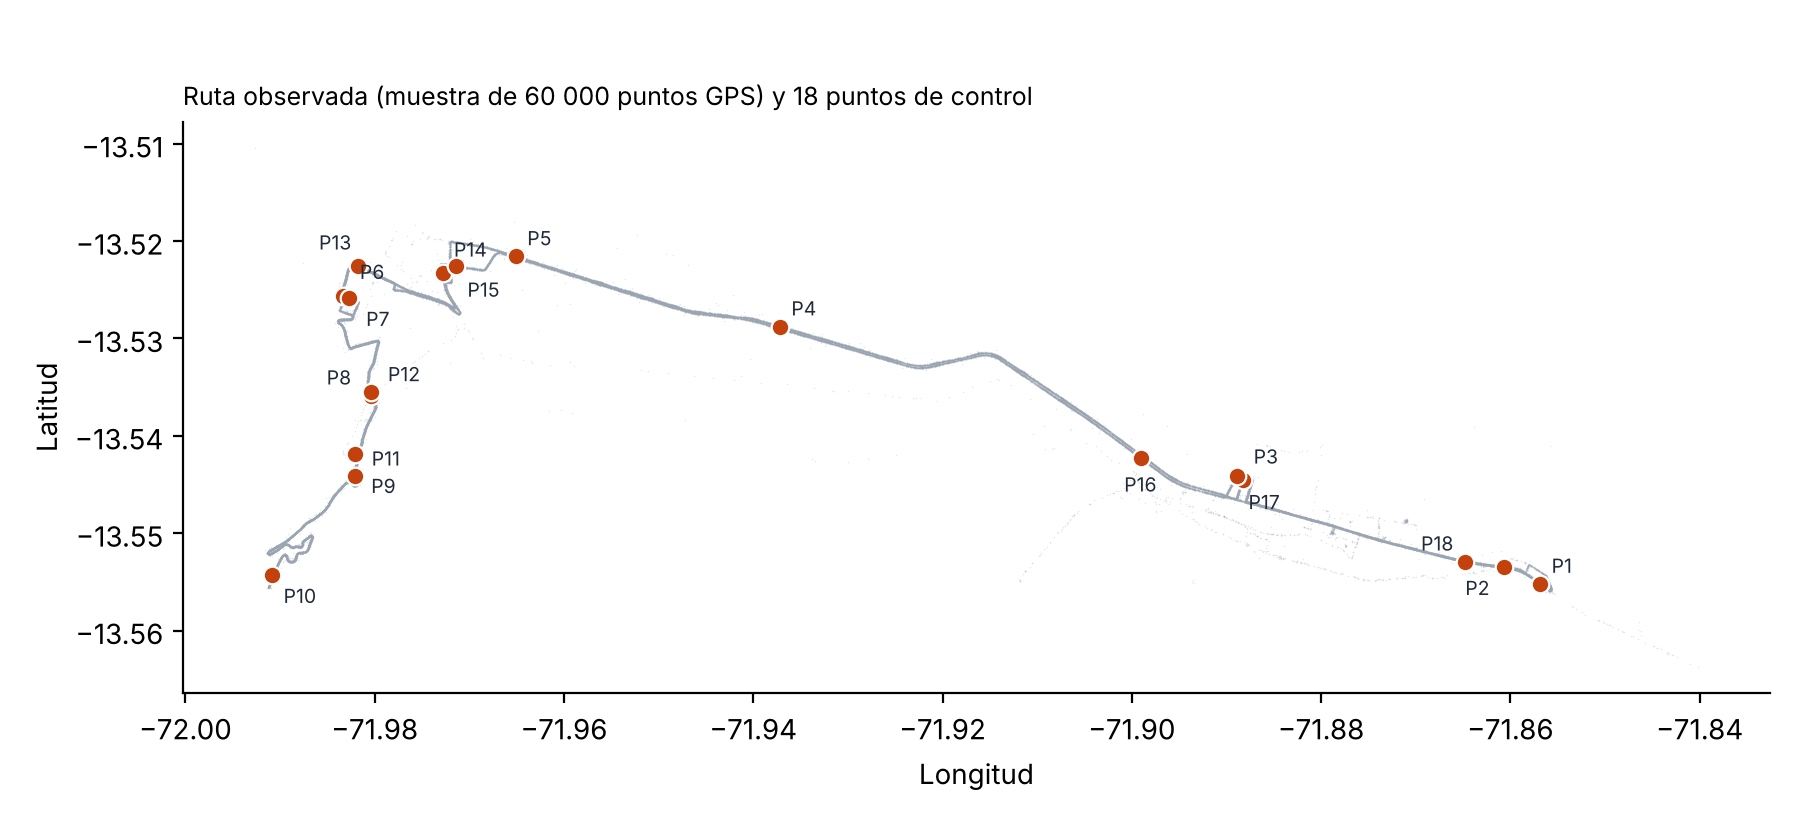
\includegraphics[width=\columnwidth]{figuras/ruta.png}
\caption{Ruta reconstruida a partir de una muestra de 60\,000 puntos GPS; cada punto de control se ubicó con la mediana de las posiciones GPS en su hora real de paso.}
\label{fig:ruta}
\end{figure}

\textbf{Calidad de datos.} Las reglas se fijaron antes de modelar y están implementadas, con aserciones, en \texttt{src/01\_preprocesamiento.py} (Tabla~\ref{tab:calidad}). Quedan 4\,559 vueltas (96,9\,\%), 4\,004 con el último punto observado: la muestra para predecir.

\begin{table}[h]
\centering
\caption{Problemas de calidad en \texttt{Times.csv} y tratamiento (sobre 4\,707 vueltas y 84\,726 pasos)}
\label{tab:calidad}
\footnotesize
\begin{tabular}{@{}p{2.3cm}p{2.5cm}p{2.9cm}@{}}
\toprule
\textbf{Problema} & \textbf{Magnitud} & \textbf{Tratamiento}\\
\midrule
Paso no registrado (``-'' y 00:00:00) & 7\,746 pasos (9,1\,\%) & NaN + indicador; el objetivo nunca se imputa\\
Horario programado no creciente & 148 vueltas (3,1\,\%) & Excluir la vuelta (arreglo corrupto)\\
Paso con hora incompatible con su vuelta ($|d|>60$ min) & 156 pasos (0,18\,\%) en 60 vueltas & Marcar el paso como NaN\\
Tramo con tiempo negativo & 30 vueltas antes de la regla anterior; 0 después & Excluir la vuelta (no se aplicó a ninguna)\\
Salto de retraso $>15$ min entre puntos consecutivos & 55 vueltas (1,2\,\%) & Conservar; solo se marca (puede ser un incidente real)\\
\bottomrule
\end{tabular}
\end{table}

\textbf{Corrección respecto a la propuesta.} En el Entregable~1, los 156 pasos con $|d|>60$ min se atribuyeron a cruces de medianoche. Ninguno está cerca de $\pm1\,440$ min, lo que produciría un cruce de medianoche. De los 141 negativos, 122 tienen una hora de reloj entre las 4 y las 6 h, y 126 de los 156 pertenecen a vueltas que salen entre las 16 y las 20 h; por ejemplo, una vuelta que sale a las 18:52 registra en P18 la hora 05:45:20. Solo el 13\,\% de esas horas queda a menos de 2 min de un paso de otra vuelta del mismo bus, frente al 33\,\% en pasos válidos desplazados al azar, de modo que no se pudo verificar que sean pasos de otra vuelta. El tratamiento no cambia (marcarlos como NaN), pero sí su justificación. Además, 93 pasos tienen $30<|d|\le60$ min; bajar el umbral a 30 min no cambia los resultados (Sección~\ref{sec:robustez}).

\textbf{Otros hallazgos.} (i) Hay 106 huecos en la numeración de vueltas entre 3\,522 pares consecutivos del mismo bus y día; el número de vuelta es poco fiable. (ii) En P18, 229 de las 642 vueltas con la plantilla de 147 min (36\,\%) llegan más de 10 min adelantadas; salen entre las 4 y las 6 h. (iii) La plantilla de 170 min (salidas de 16 a 20 h) aparece solo hasta el 24 de enero; desde el 27, esa franja usa una plantilla nueva de 168 min que no existe en el desarrollo (234 vueltas de prueba).

\textbf{Análisis exploratorio.} Se hace solo sobre el desarrollo (3\,465 vueltas; 3\,082 con P18). El retraso mediano oscila entre $-1{,}6$ y 1,6 min hasta P13, salta a 3,7 min en P14 y queda en 2,4 min en P18; el p90 pasa de 7,7 min en P13 a 12,4 en P14 (Fig.~\ref{fig:eda_punto}). El retraso en P18 depende sobre todo de la hora de salida: es negativo de madrugada (plantilla de 147 min) y cercano a cero a mediodía (Fig.~\ref{fig:eda_p18}). Por día, el sábado se separa claramente: mediana de 10,8 min frente a 1,1--2,5 min de los demás días.

\begin{figure}[t]
\centering
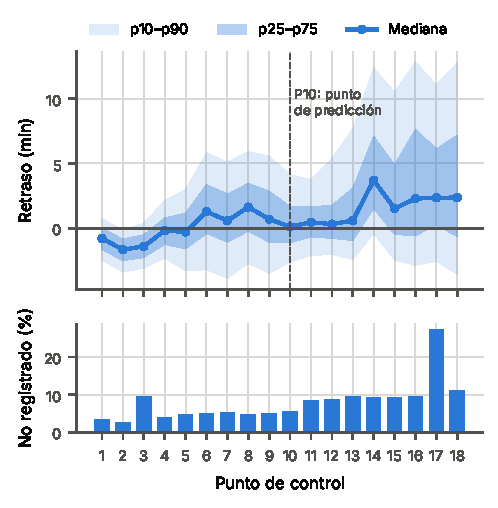
\includegraphics[width=\columnwidth]{figuras/eda_por_punto.pdf}
\caption{Desarrollo (6--26 ene): 3\,465 de las 4\,559 vueltas conservadas. Arriba: retraso por punto de control (mediana, rango intercuartílico y p10--p90). Abajo: porcentaje de pasos no registrados.}
\label{fig:eda_punto}
\end{figure}

\begin{figure*}[t]
\centering
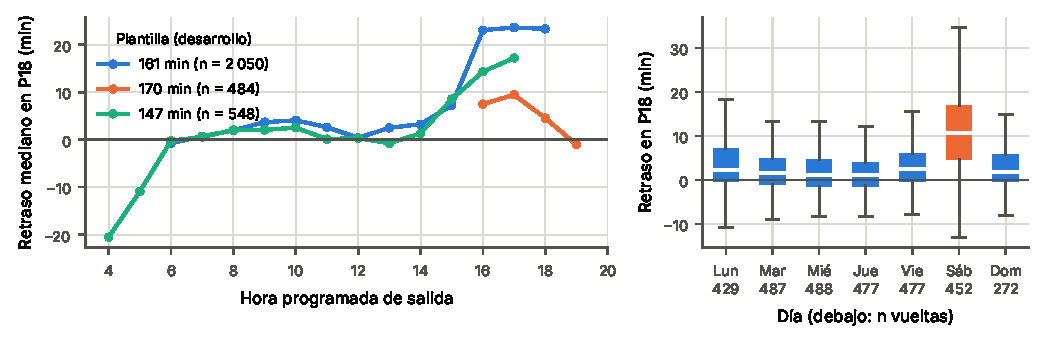
\includegraphics[width=\textwidth]{figuras/eda_p18.pdf}
\caption{Retraso en P18 en el desarrollo: 3\,082 de las 4\,004 vueltas con P18 observado. Izquierda: mediana por hora programada de salida y plantilla (se omiten horas con menos de 10 vueltas; la plantilla de 168 min no aparece en el desarrollo). Derecha: distribución por día de la semana, sin valores atípicos; el sábado se resalta.}
\label{fig:eda_p18}
\end{figure*}

% ═══════════════════════════════════════════════════════════════════════════════
\section{Metodología}

La Fig.~\ref{fig:pipeline} resume el flujo de trabajo.

\begin{figure}[t]
\centering
\resizebox{\columnwidth}{!}{%
\begin{tikzpicture}[>=Latex,
box/.style={draw, rounded corners=2pt, align=center, font=\footnotesize, minimum height=9mm, text width=23mm, fill=gray!8}]
\node[box] (a) at (0,1.0) {\texttt{Times.csv}\\18 puntos};
\node[box] (b) at (0,-0.3) {\texttt{Monitoring.csv}\\GPS};
\node[box] (c) at (3.2,0.35) {Limpieza con reglas\\cuantificadas};
\node[box] (d) at (6.4,0.35) {Variables causales en P10\\+ tiempo real};
\node[box] (e) at (6.4,-1.75) {Líneas base, Ridge,\\RF, HistGB};
\node[box] (f) at (3.2,-1.75) {CV \textit{forward-chaining}\\por días; prueba única};
\node[box] (g) at (0,-1.75) {Regresión, clases,\\grupos y demo};
\draw[->] (a) -- (c);
\draw[->] (b) -- (c);
\draw[->] (b.east) to[out=0,in=200] (d.south west);
\draw[->] (c) -- (d);
\draw[->] (d) -- (e);
\draw[->] (e) -- (f);
\draw[->] (f) -- (g);
\end{tikzpicture}}
\caption{Flujo de trabajo.}
\label{fig:pipeline}
\end{figure}

\subsection{Variable objetivo}\label{sec:objetivo}
El objetivo es $d_{\ell,18}$, el retraso de la vuelta en P18: hora real menos hora programada, en minutos con segundos. Se construye con \texttt{start\_time} (programada) y \texttt{end\_time} (real); no se usa \texttt{difference\_time} directamente porque es el mismo retraso truncado al minuto (verificado en el 100\,\% de los pasos), y el retraso con segundos tiene más resolución con el mismo significado. Se elige el retraso, y no la hora de llegada, porque es la medida que el operador controla y sanciona, y porque la llegada se recupera como hora programada más retraso predicho \cite{hu2022deepreta,wang2018wdr}. Se elige P18 porque es donde el retraso ya se acumuló (en el desarrollo, mediana de 2,4 min, desviación estándar de 8,6 y p90 de 12,8), y P10 porque a mitad de ruta quedan 8 puntos de control para actuar; la Sección~\ref{sec:curva} cuantifica cómo cambia el error con ese punto de partida. El objetivo nunca se imputa: solo las 4\,004 vueltas con P18 observado entran a la regresión, y el sesgo de excluir el resto se analiza en la Sección~\ref{sec:robustez}. Para la clasificación, el mismo retraso se convierte en tres clases (Sección~\ref{sec:clases}).

\subsection{Variables}\label{sec:variables}
Todas las variables están disponibles cuando el bus pasa por P10. El instante de decisión $t$ es la hora real de paso por P10 (si no se registró, la hora programada más el último retraso observado).
\begin{itemize}
    \item \emph{Propagación:} retrasos $d_1,\dots,d_{10}$ (NaN si el paso no se registró), último retraso observado, su variación y número de pasos faltantes.
    \item \emph{Horario:} hora programada de salida (seno y coseno), plantilla y tiempo programado restante hasta P18.
    \item \emph{Calendario y operación:} día de la semana, número de vuelta y vehículo (45, con 39--91 vueltas de desarrollo cada uno).
    \item \emph{Tiempo real, otras vueltas:} media del retraso ganado entre P10 y P14 ($d_{14}-d_{10}$) por las vueltas, de cualquier bus, que pasaron por P14 en $(t-30, t]$ min, y lo mismo para el tramo P14--P18; y cuántas vueltas aportan a cada media. Es el ``bus precedente'' de la propuesta: son tramos que esas vueltas ya terminaron antes de $t$.
    \item \emph{Tiempo real, GPS adelante:} velocidad media de los otros buses que en $(t-15, t]$ min estaban entre P10 y P14 (y entre P14 y P18). Un punto GPS está en el tramo si su bus ya había pasado el punto inicial y aún no el final, según sus propias horas reales.
    \item \emph{GPS propio:} velocidad media y fracción de puntos detenidos ($\le2$ km/h) del mismo bus entre P5 y P10.
\end{itemize}
Las ventanas (30 y 15 min) se fijaron antes de medir el error. Con unos 10 buses por hora, la ventana de 30 min reúne en mediana 5 vueltas; la media queda sin definir (NaN) en el 3\,\% de las vueltas para P10--P14 y en el 7\,\% para P14--P18.

\subsection{Modelos}
\begin{itemize}
    \item \emph{Líneas base:} retraso cero (horario perfecto); persistencia (el último retraso observado se mantiene hasta P18); media histórica del retraso en P18 por hora de salida, calculada solo con el entrenamiento de cada pliegue.
    \item \emph{Ridge:} imputación por mediana con indicadores de faltante, estandarización y \textit{one-hot} del vehículo y del día.
    \item \emph{Random Forest} \cite{breiman2001}: imputación por mediana con indicadores; 300 árboles.
    \item \emph{HistGradientBoosting} (\textit{gradient boosting} con histogramas de scikit-learn, análogo a LightGBM \cite{ke2017}): maneja los NaN de forma nativa, con el vehículo y el día como categóricas.
\end{itemize}
Toda imputación, escalado y codificación está dentro de un \textit{pipeline} que se ajusta solo con el entrenamiento de cada pliegue \cite{pedregosa2011,kaufman2012}. Se descartaron SVR, Lasso, el MLP y la LSTM de la propuesta: con unas 4\,000 vueltas y datos tabulares, los ensambles de árboles son la referencia fuerte \cite{grinsztajn2022}, y comparar muchos modelos sobre 6 días de prueba produciría diferencias indistinguibles del ruido.

\subsection{Diseño experimental}
\textbf{Partición.} Cada vuelta se asigna por su fecha de salida y nunca se divide. Desarrollo: 6--26 de enero (21 días, 3\,082 vueltas con P18). Prueba: 27 de enero--1 de febrero (6 días de lunes a sábado, 922 vueltas).

\textbf{Validación cruzada \textit{forward-chaining} por días.} El primer pliegue entrena con los primeros 11 días y valida con los 2 siguientes; cada pliegue posterior añade esos 2 días al entrenamiento. Son 5 pliegues, con 1\,655--2\,836 vueltas de entrenamiento y 225--331 de validación; nunca se valida con días anteriores a los de entrenamiento \cite{bergmeir2012}.

\textbf{Selección de variables.} Cada grupo de variables en tiempo real se añadió por separado a las 20 variables base. La regla, fijada antes de calcularla, fue incluir un grupo solo si bajaba el MAE de validación cruzada en al menos dos de los tres modelos. La misma regla descartó en el E2 el retraso de la vuelta anterior del mismo bus.

\textbf{Ajuste de hiperparámetros.} Búsqueda aleatoria que minimiza el MAE medio de los 5 pliegues: 40 configuraciones para cada ensamble y 30 para Ridge (Tabla~\ref{tab:hiper}). Luego cada modelo se reentrena con todo el desarrollo y se evalúa una vez en la prueba.

\begin{table}[h]
\centering
\caption{Hiperparámetros de regresión: espacio de búsqueda y valor elegido con las variables finales}
\label{tab:hiper}
\scriptsize
\begin{tabular}{@{}p{1.1cm}p{2.8cm}p{2.6cm}p{0.9cm}@{}}
\toprule
\textbf{Modelo} & \textbf{Parámetro} & \textbf{Espacio} & \textbf{Elegido}\\
\midrule
Ridge & $\alpha$ & log-uniforme $[10^{-3},10^{3}]$ & 1,22\\
\midrule
Random & \texttt{max\_depth} & \{None, 6, 10, 16\} & None\\
Forest & \texttt{min\_samples\_leaf} & \{1, 2, 5, 10, 20\} & 1\\
 & \texttt{max\_features} & \{0,3; 0,5; 0,8; 1,0\} & 0,5\\
\midrule
HistGB & \texttt{learning\_rate} & log-uniforme $[0{,}01;0{,}2]$ & 0,034\\
 & \texttt{max\_iter} & \{100, 200, 400, 800\} & 400\\
 & \texttt{max\_leaf\_nodes} & \{7, 15, 31, 63\} & 7\\
 & \texttt{min\_samples\_leaf} & \{5, 10, 20, 40\} & 40\\
 & \texttt{l2\_regularization} & log-uniforme $[10^{-3},10]$ & 0,0099\\
\bottomrule
\end{tabular}
\end{table}

\textbf{Uso de la prueba.} Los resultados preliminares del E1 ya se calcularon sobre el mismo periodo de prueba. Desde el E2, todas las decisiones (limpieza, variables, hiperparámetros, umbrales) se toman solo con validación cruzada. En el E2, el protocolo se congeló en un \textit{commit} (\texttt{6445b10}) y los modelos con solo el registro de horarios se evaluaron una vez. En esta entrega, los modelos nuevos se evaluaron también una sola vez; antes de hacerlo se registró la huella SHA-256 del código y los datos (\texttt{8758d774385dea67}) y el script se niega a repetir la evaluación. Los modelos del E2 no se reevaluaron: se comparan con sus predicciones guardadas. Una salvedad: la idea de modelar el estado del tramo P10--P14 surgió del análisis del E2, que incluyó el desglose del error en la prueba, así que la prueba no es completamente ciega para esta entrega.

\subsection{Clasificación de puntualidad}\label{sec:clases}
La clase de la vuelta en P18 sigue la convención de TCRP \cite{tcrp2003}: adelantada si $d_{18}<-1$ min, puntual si $-1\le d_{18}\le5$ y retrasada si $d_{18}>5$. En el desarrollo, el reparto es 22\,\%, 44\,\% y 34\,\%. Desde P10, con las mismas variables y pliegues, se comparan la clase mayoritaria, la persistencia (la clase del último retraso observado), regresión logística, Random Forest y HistGradientBoosting (estos tres con pesos de clase balanceados y búsqueda aleatoria de 20--30 configuraciones que maximiza el F1 macro), y el HistGB de regresión final con sus predicciones convertidas en clase con los mismos umbrales. La métrica principal es el F1 macro, porque las tres clases importan por igual al despachador; se reportan también la exactitud balanceada y la exactitud.

\subsection{Agrupamiento de perfiles de retraso}
Cada vuelta del desarrollo con los 18 retrasos observados (2\,361 vueltas) es un perfil de 18 valores en minutos. Se comparan K-means (20 inicializaciones) y una mezcla gaussiana de covarianza completa con $k=2,\dots,8$. El número de grupos se elige con el coeficiente de silueta; se reportan también el índice de Davies-Bouldin y el BIC de la mezcla. PCA a dos componentes se usa solo para visualizar. Las 708 vueltas de prueba con perfil completo se asignan al centroide más cercano, sin reajustar, para ver en qué grupos se concentra el error de la regresión.

\subsection{Métricas y comparación estadística}
\begin{itemize}
    \item \emph{Regresión:} MAE en minutos (principal), RMSE, $R^2$ y porcentaje de predicciones con error absoluto $\le2$ min (operativa).
    \item \emph{Intervalos de confianza del 95\,\%:} \textit{bootstrap} por día (2\,000 remuestreos de los 6 días de prueba), porque las vueltas de un mismo día comparten tráfico y no son independientes. Con solo 6 días, son aproximados.
    \item \emph{Comparación entre modelos:} la unidad es el día. Para cada alternativa se reporta la diferencia de MAE con el mejor modelo, su IC por \textit{bootstrap} pareado por día (5\,000 remuestreos) y una prueba de signo sobre los 6 días, que no puede bajar de $p=0{,}03$.
\end{itemize}

% ═══════════════════════════════════════════════════════════════════════════════
\section{Experimentos y Resultados}\label{sec:resultados}

\subsection{Selección de las variables en tiempo real}
La Tabla~\ref{tab:ablacion} muestra la ablación. Las variables de otras vueltas bajan el MAE en los tres modelos, sobre todo en Ridge (3,79 $\to$ 3,61 min). La velocidad GPS de los buses que van adelante lo baja en dos de tres. El GPS del propio bus solo lo baja en Ridge, de modo que no se incluye: la trayectoria del bus hasta P10 ya está resumida en sus retrasos observados. Las diferencias en los ensambles (0,02--0,05 min) son pequeñas frente a la desviación entre pliegues (alrededor de 0,9 min).

\begin{table}[h]
\centering
\caption{Ablación de las variables en tiempo real: MAE de validación cruzada (min) con los hiperparámetros del E2}
\label{tab:ablacion}
\footnotesize
\begin{tabular}{@{}lccc@{}}
\toprule
\textbf{Variables} & \textbf{Ridge} & \textbf{RF} & \textbf{HistGB}\\
\midrule
Base (20 variables del registro de horarios) & 3,79 & 3,53 & 3,375\\
+ otras vueltas (precedentes) & \textbf{3,61} & \textbf{3,48} & \textbf{3,356}\\
+ GPS de los buses adelante & 3,74 & 3,56 & 3,370\\
+ GPS del propio bus & 3,77 & 3,54 & 3,376\\
\bottomrule
\end{tabular}
\end{table}

\subsection{Validación cruzada}
Con los dos grupos elegidos (26 variables) y la nueva búsqueda de hiperparámetros, los tres modelos superan a las tres líneas base y HistGB obtiene el menor MAE (Tabla~\ref{tab:cv}). La búsqueda de HistGB eligió la misma configuración que en el E2. La mejora por las variables en tiempo real es grande en Ridge (0,19 min) y pequeña en los ensambles (0,04--0,06 min).

\begin{table}[h]
\centering
\caption{Validación cruzada \textit{forward-chaining} (media $\pm$ desviación estándar en 5 pliegues). TR: con variables en tiempo real}
\label{tab:cv}
\footnotesize
\begin{tabular}{@{}lcccc@{}}
\toprule
\textbf{Modelo} & \textbf{MAE} & \textbf{RMSE} & \textbf{$R^2$} & \textbf{$\le$2 min}\\
\midrule
Retraso cero & 7,28 $\pm$ 2,87 & 9,95 & $-0{,}29$ & 27\,\%\\
Persistencia & 5,49 $\pm$ 1,58 & 7,26 & 0,31 & 29\,\%\\
Media histórica por hora & 5,01 $\pm$ 2,32 & 6,77 & 0,41 & 32\,\%\\
Ridge & 3,79 $\pm$ 0,72 & 5,03 & 0,66 & 34\,\%\\
Random Forest & 3,53 $\pm$ 1,03 & 4,91 & 0,69 & 40\,\%\\
HistGB & 3,38 $\pm$ 0,95 & 4,70 & 0,71 & 42\,\%\\
Ridge + TR & 3,60 $\pm$ 0,69 & 4,84 & 0,68 & 38\,\%\\
Random Forest + TR & 3,47 $\pm$ 0,95 & 4,82 & 0,69 & 41\,\%\\
HistGB + TR & \textbf{3,34} $\pm$ 0,86 & \textbf{4,67} & \textbf{0,71} & \textbf{42}\,\%\\
\bottomrule
\end{tabular}
\end{table}

\subsection{Evaluación final en la prueba}
La Tabla~\ref{tab:test} reúne la evaluación única de los modelos del E2 y la de los modelos nuevos.
\begin{itemize}
    \item HistGB con variables en tiempo real obtiene el menor error: MAE de 2,76 min, un 36\,\% menos que la persistencia (4,32 min), con $R^2=0{,}76$ y un 50\,\% de predicciones con error de 2 min o menos.
    \item Frente al HistGB del E2, sin tiempo real, la diferencia es de 0,01 min (IC $-0{,}06$ a 0,11) y cada uno gana en 3 de los 6 días: en la prueba, las variables en tiempo real no mejoran a HistGB en conjunto.
    \item Sí mejoran a Ridge (3,41 $\to$ 3,22 min), en línea con la validación cruzada.
\end{itemize}

\begin{table*}[t]
\centering
\caption{Prueba (27 ene--1 feb 2025, 922 vueltas). Cada modelo se evaluó una sola vez: los de solo horarios en el E2 y los de tiempo real (TR) en esta entrega. Entre corchetes, IC del 95\,\% por \textit{bootstrap} por día. $\Delta$MAE: cuánto mayor es el MAE de cada modelo que el del HistGB + TR, con su IC y en cuántos de los 6 días HistGB + TR tiene menor MAE. $^\dagger$Línea base añadida en la revisión del E2, después de la evaluación única.}
\label{tab:test}
\footnotesize
\begin{tabular}{@{}lccccc@{}}
\toprule
\textbf{Modelo} & \textbf{MAE (min)} & \textbf{RMSE (min)} & \textbf{$R^2$} & \textbf{Error $\le$ 2 min} & \textbf{$\Delta$MAE vs.\ HistGB + TR [IC] (días)}\\
\midrule
Retraso cero & 5,61 [4,16; 8,65] & 8,51 & $-0{,}07$ [$-0{,}28$; $-0{,}01$] & 36\,\% & ---\\
Persistencia & 4,32 [3,37; 6,19] & 6,15 & 0,44 [0,34; 0,52] & 36\,\% & +1,56 [0,90; 2,94] (6/6)\\
Media histórica por hora & 4,44 [3,55; 6,28] & 6,17 & 0,44 [0,35; 0,50] & 34\,\% & ---\\
Media por hora y tipo de día$^\dagger$ & 3,34 & 4,76 & 0,67 & 43\,\% & ---\\
\midrule
Ridge & 3,41 [2,97; 4,03] & 4,61 & 0,69 [0,50; 0,78] & 38\,\% & ---\\
Random Forest & 2,97 [2,52; 3,75] & 4,32 & 0,72 [0,60; 0,79] & 48\,\% & ---\\
HistGB & 2,77 [2,29; 3,44] & 4,04 & 0,76 [0,62; 0,83] & 49\,\% & +0,01 [$-0{,}06$; 0,11] (3/6)\\
\midrule
Ridge + TR & 3,22 [2,86; 3,71] & 4,44 & 0,71 [0,53; 0,80] & 40\,\% & +0,46 [0,13; 0,70] (5/6)\\
Random Forest + TR & 2,94 [2,57; 3,59] & 4,21 & 0,74 [0,58; 0,81] & 45\,\% & +0,18 [$-0{,}06$; 0,37] (5/6)\\
HistGB + TR & \textbf{2,76} [2,28; 3,34] & \textbf{4,00} & \textbf{0,76} [0,62; 0,84] & \textbf{50}\,\% & ---\\
\bottomrule
\end{tabular}
\end{table*}

\textbf{Metas.} (i) Superar a la mejor línea base en MAE: se cumple. HistGB + TR tiene menor MAE que la persistencia en los 6 días (diferencia de 1,56 min, IC 0,90--2,94; prueba de signo $p=0{,}03$) y también que la línea base por hora y tipo de día (3,34 min). (ii) $R^2\ge0{,}80$ desde P10: no se demuestra. La estimación queda por debajo en validación cruzada ($0{,}71\pm0{,}05$; ningún pliegue llega a 0,80, el máximo es 0,78) y en la prueba (0,76); con 6 días, el IC (0,62--0,84) no permite confirmarla ni descartarla. (iii) Como medida complementaria del umbral del 80\,\%, calculada después de la evaluación única con las predicciones guardadas (\texttt{src/13\_metricas\_umbral.py}), el 86\,\% de las predicciones de prueba tiene un error absoluto de 5 min o menos (80\,\% en validación cruzada, con desviación de 10 puntos entre pliegues), frente al 69\,\% de la persistencia. El umbral de 5 min es el de la convención de puntualidad de TCRP \cite{tcrp2003}, no se eligió a partir de los resultados.

\subsection{Comparación estadística por día}\label{sec:comparacion}
\begin{itemize}
    \item HistGB + TR tiene menor MAE que la persistencia en los 6 días y que Ridge + TR en 5 (IC de la diferencia 0,13--0,70).
    \item Frente a Random Forest + TR, la diferencia es pequeña (0,18 min) y su IC incluye el 0. En el E2, sin tiempo real, HistGB superaba a Random Forest por 0,20 min (IC 0,02--0,37) en 5 de 6 días, con prueba de signo $p=0{,}22$. La ventaja de HistGB sobre Random Forest es consistente en el signo pero no concluyente.
    \item La prueba de Wilcoxon por vuelta de la propuesta trata como independientes vueltas que no lo son y daba valores $p$ demasiado optimistas ($9\times10^{-5}$); por eso la unidad es el día.
\end{itemize}

\subsection{Dónde aportan las variables en tiempo real}
La Fig.~\ref{fig:dia} muestra el MAE por día. El sábado 1 de febrero, el día con más error, HistGB + TR baja de 4,61 a 4,30 min. De lunes a viernes los dos HistGB quedan muy cerca (el lunes, 3,24 frente a 3,14 min). En las vueltas con la plantilla nueva de 168 min, el MAE baja de 3,37 a 3,28 min. La importancia por permutación (Fig.~\ref{fig:imp}) explica el patrón: con las variables en tiempo real, el día de la semana pasa de 0,74 a 0,41 min de aumento del MAE, y la ganancia P10--P14 de las vueltas precedentes ocupa el cuarto lugar (0,28 min). El modelo sustituye en parte el ``calendario'' por la congestión observada. La velocidad GPS casi no aporta una vez incluida esa ganancia (0,01 min).

\begin{figure}[t]
\centering
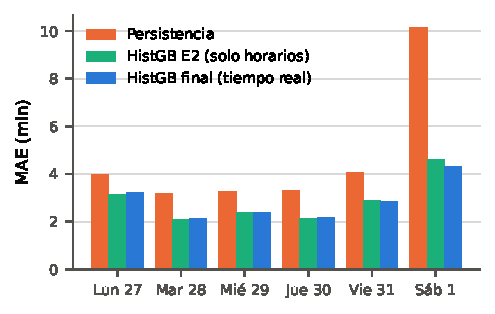
\includegraphics[width=\columnwidth]{figuras/final_por_dia.pdf}
\caption{MAE por día de prueba de la persistencia, el HistGB del E2 (solo horarios) y el HistGB final (con tiempo real).}
\label{fig:dia}
\end{figure}

\begin{figure}[t]
\centering
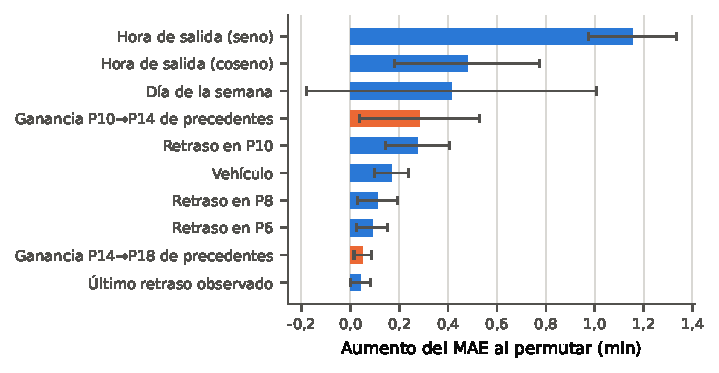
\includegraphics[width=\columnwidth]{figuras/final_importancia.pdf}
\caption{Importancia por permutación del HistGB final: aumento medio del MAE en los 5 pliegues de validación al desordenar cada variable (10 repeticiones); barras de error: $\pm1$ desviación estándar. En naranja, las variables en tiempo real.}
\label{fig:imp}
\end{figure}

\subsection{Desglose del error en la prueba}\label{sec:desglose}
\begin{itemize}
    \item \emph{Sábado.} Es el 11\,\% de las vueltas de prueba y aportaba el 19\,\% del error absoluto del HistGB del E2. Ese día el retraso medio subió de 3,6 a 14,7 min entre P10 y P14, y el retraso mediano en P18 fue de 14,2 min, frente a 0,6--1,6 min de lunes a viernes. Incluso el retraso cero tiene un MAE de 15,2 min. El modelo vio solo tres sábados en el desarrollo y subestima sus retrasos grandes.
    \item \emph{Horario nuevo.} Las vueltas de lunes a viernes con la plantilla de 168 min son el 19\,\% de la prueba y aportaban el 24\,\% del error. Su MAE (3,28 min) es mayor que con la plantilla de 161 min (2,66), pero el modelo no colapsa: la hora de salida, su variable más importante, sí está representada. Sigue muy por debajo de la persistencia en esas vueltas (4,91 min).
    \item \emph{$R^2$ por subgrupo.} El $R^2$ depende de la varianza de cada grupo: en el E2, el sábado, con el mayor MAE (4,61 min), tenía $R^2=0{,}73$ porque su retraso es muy variable (desviación estándar de 11,5 min), y la plantilla de 168 min, con menor MAE (3,37 min), $R^2=0{,}30$ (desviación de 5,1 min). Por eso el MAE es la métrica principal.
\end{itemize}

\subsection{Error según el punto de partida}\label{sec:curva}
Para cada punto de partida $k=5,\dots,17$ se repitió la validación cruzada con las variables del registro de horarios, ahora con una búsqueda de hiperparámetros propia para cada $k$ (20 configuraciones para HistGB y 15 para Ridge); la prueba no se usó (Fig.~\ref{fig:curva}).
\begin{itemize}
    \item HistGB tiene el menor MAE hasta P15. Su ventaja sobre la persistencia es grande al inicio (3,55 frente a 6,82 min en P5) y desaparece al final (1,49 frente a 1,65 min en P16).
    \item La mejora es gradual hasta P12 (3,14 min) y se acelera entre P12 y P14 (2,67 min), justo donde el EDA muestra el salto del retraso.
    \item \emph{La meta $R^2\ge0{,}80$ se alcanza desde P14} ($R^2=0{,}81\pm0{,}04$); desde P10 el modelo se queda en $0{,}71\pm0{,}06$.
    \item Ajustar los hiperparámetros para cada $k$ cambia el MAE en 0,07 min o menos frente a reutilizar los de $k=10$, muy por debajo de la desviación entre pliegues. La mayor mejora está en P16--P17 (1,56 $\to$ 1,49 y 1,32 $\to$ 1,24 min), pero ahí Ridge sigue siendo ligeramente mejor (1,47 y 1,14 min): cerca del final, el retraso restante es casi lineal en el último retraso observado.
\end{itemize}

\begin{figure*}[t]
\centering
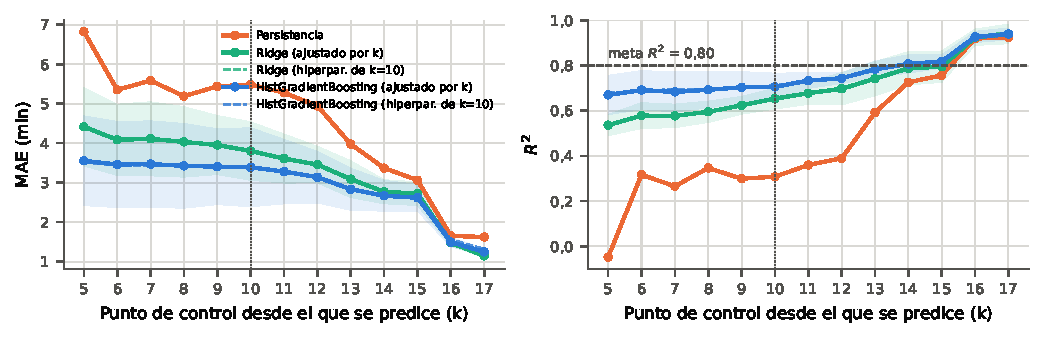
\includegraphics[width=\textwidth]{figuras/final_curva_k.pdf}
\caption{MAE y $R^2$ en validación cruzada según el punto de control desde el que se predice el retraso en P18 (media de 5 pliegues; banda: $\pm1$ desviación estándar). Líneas continuas: hiperparámetros ajustados para cada $k$; discontinuas: hiperparámetros de $k=10$ (E2). La línea vertical marca el experimento principal.}
\label{fig:curva}
\end{figure*}

\subsection{Clasificación de puntualidad}\label{sec:clasif}
La Tabla~\ref{tab:clasif} muestra la clasificación. En validación cruzada, el mejor F1 macro lo obtiene el HistGB de regresión con sus predicciones convertidas en clase (0,69), seguido de cerca por los clasificadores Random Forest y HistGB (0,68). Ese modelo, elegido sin mirar la prueba, también es el mejor en ella: F1 macro de 0,70 (IC 0,62--0,77), frente a 0,50 de la persistencia y 0,22 de la clase mayoritaria. Que un regresor bien ajustado supere a clasificadores entrenados para la tarea indica que las clases solo agregan información que ya está en el retraso predicho.

\begin{table}[h]
\centering
\caption{Clasificación de puntualidad en P18 desde P10 (adelantada $<-1$ min, puntual, retrasada $>5$ min). Prueba: 233, 438 y 251 vueltas. Entre corchetes, IC del 95\,\% por día}
\label{tab:clasif}
\footnotesize
\begin{tabular}{@{}lccc@{}}
\toprule
 & \textbf{CV} & \multicolumn{2}{c}{\textbf{Prueba}}\\
\textbf{Modelo} & \textbf{F1 macro} & \textbf{F1 macro} & \textbf{Exact. bal.}\\
\midrule
Clase mayoritaria & 0,19 & 0,22 [0,17; 0,24] & 0,33\\
Persistencia & 0,46 & 0,50 [0,40; 0,58] & 0,51\\
Regresión logística & 0,65 & 0,65 [0,58; 0,73] & 0,66\\
Random Forest & 0,68 & 0,66 [0,60; 0,72] & 0,66\\
HistGB (clasificador) & 0,68 & 0,69 [0,63; 0,75] & 0,69\\
HistGB regresión + umbrales & \textbf{0,69} & \textbf{0,70} [0,62; 0,77] & \textbf{0,69}\\
\bottomrule
\end{tabular}
\end{table}

La matriz de confusión (Fig.~\ref{fig:cm}) muestra que el error grave es raro: de 251 vueltas retrasadas, ninguna se predijo adelantada, y solo 8 de 233 adelantadas se predijeron retrasadas. El modelo detecta el 80,5\,\% de las vueltas retrasadas (202 de 251), y cuando predice ``retrasada'' acierta en el 69\,\% de los casos. La exactitud global es del 70,7\,\%, por debajo del 80\,\%. La clase más difícil es ``adelantada'': solo detecta el 52\,\%, y el resto lo predice como puntual, porque el adelanto final suele ser pequeño y cercano al umbral de $-1$ min.

\begin{figure}[t]
\centering
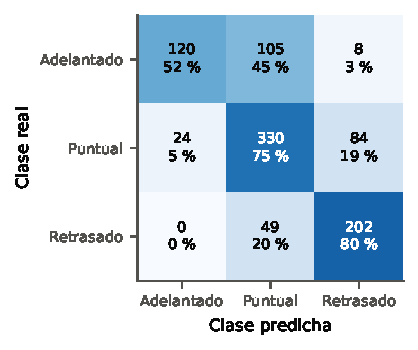
\includegraphics[width=0.8\columnwidth]{figuras/final_matriz_confusion.pdf}
\caption{Matriz de confusión en la prueba del HistGB de regresión convertido en clases (elegido por F1 macro en validación cruzada). Porcentajes por fila (clase real).}
\label{fig:cm}
\end{figure}

\subsection{Agrupamiento de perfiles de retraso}\label{sec:grupos}
El coeficiente de silueta de K-means es máximo con $k=2$ (0,69; Davies-Bouldin 0,43) y baja a 0,54 con $k=3$ y a 0,30 o menos con $k\ge4$. La mezcla gaussiana da peor silueta para todo $k\ge3$, y su BIC mínimo ($k=5$) corresponde a grupos muy solapados (silueta 0,07), así que se mantiene K-means. Con $k=2$ solo se separa un grupo pequeño de vueltas adelantadas. Con $k=3$, la solución que ya se observó en la propuesta, aparecen tres perfiles interpretables (Fig.~\ref{fig:grupos}):
\begin{itemize}
    \item \emph{Normal} (79\,\%): retraso cercano a 0 en toda la ruta y 1,5 min de media en P18.
    \item \emph{Adelantado} (7\,\%): el adelanto crece desde P4 y llega a $-18$ min en P18; salen de madrugada (hora media 5,1 h) con la plantilla de 147 min. Es el horario que sobreestima el tiempo de viaje.
    \item \emph{Retraso alto} (14\,\%): el retraso salta entre P12 y P14 hasta unos 14 min y se mantiene. El 72\,\% de estas vueltas son de sábado.
\end{itemize}
Las dos primeras componentes principales explican el 83\,\% y el 7\,\% de la varianza; la primera ordena los perfiles de adelantado a retrasado. En la prueba, la proporción de cada grupo se mantiene (80\,\%, 9\,\% y 11\,\%). El error se concentra en el grupo de retraso alto: MAE de 4,84 min con HistGB + TR, frente a 2,26 en los otros dos grupos. En ese grupo las variables en tiempo real ayudan (el HistGB del E2 tenía 5,26 min), y la persistencia falla por completo (11,49 min) porque en P10 el salto todavía no ha ocurrido.

\begin{figure*}[t]
\centering
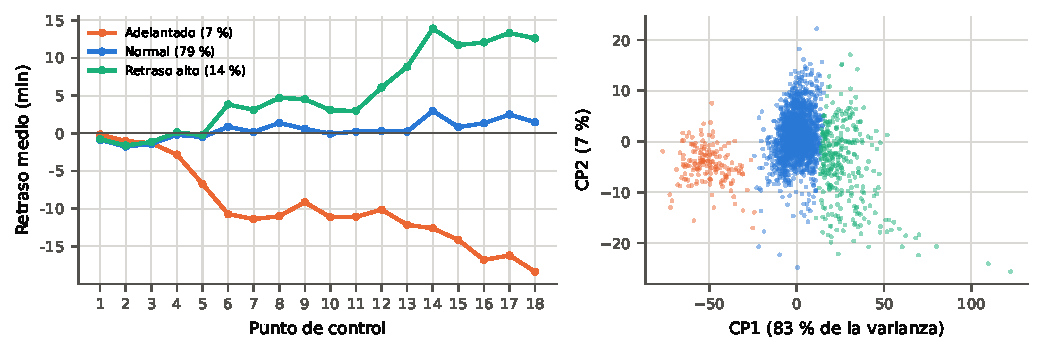
\includegraphics[width=\textwidth]{figuras/final_agrupamiento.pdf}
\caption{K-means con $k=3$ sobre los 2\,361 perfiles completos del desarrollo. Izquierda: retraso medio por punto de control de cada grupo (entre paréntesis, su porcentaje de vueltas). Derecha: proyección en las dos primeras componentes principales.}
\label{fig:grupos}
\end{figure*}

\subsection{Robustez}\label{sec:robustez}
\begin{itemize}
    \item \emph{Umbral de limpieza:} bajar el umbral de ``paso con hora incompatible'' de 60 a 30 min marca 249 pasos en lugar de 156; comparado sobre las mismas vueltas de validación, el MAE de HistGB pasa de 3,21 a 3,20 min.
    \item \emph{Hiperparámetros:} en el E2, las 5 mejores configuraciones de cada modelo difieren en menos de 0,02 min de MAE de validación cruzada, frente a unos 0,9 min de desviación entre pliegues. Frente a la configuración por defecto, el ajuste baja el MAE de HistGB en 0,11 min.
    \item \emph{Semilla:} con las semillas 0, 1 y 2, el mejor MAE de validación cruzada de HistGB varía entre 3,375 y 3,386 min, y el de Random Forest, entre 3,526 y 3,553 min.
    \item \emph{Sesgo de selección:} el 11\,\% de las vueltas de desarrollo no tiene P18 y se excluye. Salen más tarde (hora media 13,8 frente a 11,2) y algo más en sábado (18\,\% frente a 15\,\%), pero sus retrasos ya observados son similares (mediana de 3,8 frente a 3,7 min en P14).
\end{itemize}

% ═══════════════════════════════════════════════════════════════════════════════
\section{Demostración}\label{sec:demo}
La demo (\texttt{Entrega final/demo/index.html}) es un solo archivo HTML que funciona sin conexión. Permite elegir un día de prueba y una vuelta real, y avanzar el bus punto por punto sobre el mapa de la ruta reconstruido con el GPS. En cada punto muestra los retrasos observados, la predicción del retraso en P18 con su error esperado y la clase de puntualidad. Las predicciones de P5 a P17 provienen de un HistGB entrenado para cada punto de partida con los hiperparámetros de la Sección~\ref{sec:curva}; en P10 se usa el modelo final, que muestra también las variables en tiempo real (retraso ganado por los precedentes y velocidad GPS del tramo siguiente). Al llegar a P18, o con la opción ``mostrar lo que pasó'', se revela el retraso real. Todos los modelos se entrenaron solo con el desarrollo; la demo muestra predicciones sobre la prueba, pero las métricas por punto de partida se reportan solo en validación cruzada.

% ═══════════════════════════════════════════════════════════════════════════════
\section{Discusión}

\textbf{Por qué ganan los ensambles.} La persistencia supone que el retraso de P10 se mantiene, pero el retraso cambia en la segunda mitad de la ruta según la hora, la plantilla y el día. Los ensambles capturan esas interacciones, y la ganancia frente a Ridge (3,22 $\to$ 2,76 min con las mismas variables) indica que la relación no es lineal. Coincide con \cite{martyanov2026}.

\textbf{Por qué el tiempo real ayuda poco a HistGB.} El retraso ganado por los precedentes tiene una correlación de 0,54 con el cambio de retraso entre P10 y P18 en el desarrollo, pero buena parte de esa información ya estaba en la hora de salida y el día: los precedentes salen a una hora parecida el mismo día. Ridge, que no puede modelar bien las interacciones entre hora y día, aprovecha mucho la nueva variable; HistGB, que ya las capturaba, apenas. Donde la hora y el día no bastan, el sábado y el grupo de retraso alto, el tiempo real sí reduce el error. Que el modelo dependa menos del día de la semana es una ventaja práctica: ante un feriado o un evento, la congestión observada reacciona y el calendario no.

\textbf{Dónde falla el modelo.} El error se concentra en las vueltas con un salto de retraso entre P12 y P14, sobre todo los sábados. Con solo tres sábados de desarrollo, el día es la variable con menos ejemplos por categoría. La hipótesis de la congestión de fin de semana en la segunda mitad de la ruta es coherente con el perfil de retraso alto del agrupamiento. Para mitigarlo hacen falta más semanas de datos o información del tramo con más antelación.

\textbf{¿Cuánto $R^2$ es alcanzable desde P10?} La curva por punto de partida sugiere que el límite está en la información disponible y no en el modelo: el $R^2$ sube rápido solo cuando el bus ya pasó el tramo P12--P14, donde se produce la mayor parte del retraso. Las variables en tiempo real dan una visión parcial y con desfase de ese tramo, y no bastan para alcanzar la meta desde P10.

\textbf{El objetivo depende del horario.} El retraso se mide respecto a un horario que no siempre es realista: la plantilla de 147 min termina sistemáticamente adelantada, y el agrupamiento lo confirma como un grupo propio. El modelo aprende en parte a corregir el horario; si el operador lo cambia, como ocurrió al inicio de la prueba, hay que reentrenar o describir el horario por tramos.

\textbf{Uso operativo.} Con un MAE de 2,76 min, el modelo sirve para anticipar retrasos grandes con 8 puntos de antelación, no para avisos al minuto (el 50\,\% de las predicciones tiene un error de 2 min o menos). En forma de clase, detecta el 80\,\% de las vueltas que llegarán retrasadas y casi nunca confunde una retrasada con una adelantada: es el formato más útil para decidir si retener o adelantar un bus. Entrenar el modelo toma menos de un segundo y predecir una vuelta, menos de 0,01 ms.

\textbf{Comparación con la literatura.} Martyanov et al.~\cite{martyanov2026} reportan MAE $\approx$ 3,6 min y $R^2\approx$ 0,44, y Petersen et al.~\cite{petersen2019}, 1,99 min. Nuestras cifras no son directamente comparables: allí se predice para toda una red o línea y en todas las paradas; aquí, una sola ruta, un punto objetivo y un horizonte fijo, y nuestro $R^2$ se apoya en diferencias grandes y predecibles entre franjas horarias. Lo comparable es la conclusión cualitativa: los ensambles de árboles superan a la persistencia y a los modelos lineales, y la hora y la posición en la ruta dominan.

\textbf{Limitaciones y validez externa.}
\begin{itemize}
    \item Una sola ruta y 27 días: no se capturan la estacionalidad ni otras rutas.
    \item La prueba tiene 6 días y un solo sábado; los IC son aproximados y las conclusiones sobre el sábado descansan en un día.
    \item El periodo de prueba se usó en el E1, y el diagnóstico del E2 sobre la prueba motivó las variables en tiempo real.
    \item El horario de la tarde cambió al inicio de la prueba (plantilla de 168 min no vista en el desarrollo).
    \item Se excluye el 11\,\% de vueltas sin P18, que salen más tarde; el error podría estar ligeramente subestimado en las franjas más congestionadas.
    \item El agrupamiento usa solo vueltas con los 18 pasos registrados (68\,\% del desarrollo).
\end{itemize}

% ═══════════════════════════════════════════════════════════════════════════════
\section{Conclusiones y Trabajo Futuro}

Con los datos del sistema de transporte inteligente de Cusco, un HistGradientBoosting ajustado con validación temporal predice desde la mitad de la ruta el retraso en el último punto de control con un MAE de 2,76 min, un 36\,\% menos que la persistencia, y es mejor que ella en los 6 días de prueba. Se cumple la meta de superar a la mejor línea base; la de $R^2\ge0{,}80$ no se demuestra desde P10 (0,76 en la prueba) y en validación cruzada se alcanza desde P14. Las variables en tiempo real construidas con otras vueltas y el GPS mejoran claramente a Ridge, reducen el error del sábado y del grupo de retraso alto, y hacen al modelo menos dependiente del calendario, pero no mejoran el MAE global de HistGB en la prueba. Convertida en clases, la predicción alcanza un F1 macro de 0,70 y casi nunca confunde una vuelta retrasada con una adelantada. El agrupamiento revela dos fuentes de error sistemático: un horario de madrugada que sobreestima el tiempo de viaje y un salto de retraso en el tramo P12--P14, típico del sábado. La limpieza descartó que los pasos anómalos sean cruces de medianoche.

\textbf{Trabajo futuro.}
\begin{itemize}
    \item Más semanas de datos, sobre todo sábados y feriados, para modelar el fin de semana.
    \item Describir el horario por tramos para que el modelo se adapte a cambios de plantilla.
    \item Predecir todos los puntos restantes a la vez (multihorizonte) y modelar el apelotonamiento con el intervalo entre buses consecutivos.
    \item Validar la demo con despachadores y medir si la clase predicha cambia sus decisiones.
\end{itemize}

% ═══════════════════════════════════════════════════════════════════════════════
\section{Entorno Computacional y Reproducibilidad}
\begin{itemize}
    \item \emph{Entorno:} Python 3.13 con numpy 2.5.3, pandas 3.0.5, scikit-learn 1.9.1 y scipy 1.18.1 (versiones fijadas en \texttt{requirements.txt}). Los análisis de esta entrega se ejecutaron en macOS con 10 núcleos.
    \item \emph{Código:} \url{https://github.com/jeremygiraldo/1inf02-machine-learning-project}, rama \texttt{main}. Scripts en \texttt{src/}: \texttt{01} limpieza, \texttt{02} EDA, \texttt{04}--\texttt{06} regresión del E2 y su revisión, \texttt{07} variables en tiempo real, \texttt{08} ablación, ajuste, clasificación y prueba final, \texttt{09} curva por punto de partida, \texttt{10} agrupamiento, \texttt{11} demo, \texttt{12} figuras y \texttt{13} porcentaje de error dentro de 2, 3 y 5 min.
    \item \emph{Datos:} \texttt{Times.csv} está en el repositorio; \texttt{Monitoring.csv} (121 MB) no, y debe colocarse en \texttt{Dataset/}.
    \item \emph{Aleatoriedad:} semilla 42 en las búsquedas, los modelos y el \textit{bootstrap}.
    \item \emph{Prueba:} \texttt{resultados/PRUEBA\_EVALUADA.txt} (E2, \textit{commit} \texttt{6445b10}) y \texttt{resultados/PRUEBA\_FINAL\_EVALUADA.txt} (entrega final, huella \texttt{8758d774385dea67}) registran las evaluaciones únicas; los scripts se niegan a repetirlas.
\end{itemize}

\bibliographystyle{IEEEtran}
\begin{thebibliography}{99}

\bibitem{reich2019}
T.~Reich, M.~Budka, D.~Robbins, and D.~Hulbert,
``Survey of ETA prediction methods in public transport networks,''
arXiv:1904.05037, 2019.

\bibitem{kumar2025review}
B.~A. Kumar, R.~Singh, H.~E. Shaji, and L.~Vanajakshi,
``Bus arrival time prediction: A comprehensive review,''
\textit{IEEE Trans. Intell. Transp. Syst.}, vol.~26, no.~6, 2025.

\bibitem{chien2002}
S.~I.-J. Chien, Y.~Ding, and C.~Wei,
``Dynamic bus arrival time prediction with artificial neural networks,''
\textit{J. Transp. Eng.}, vol.~128, no.~5, pp. 429--438, 2002.

\bibitem{jeong2004}
R.~Jeong and L.~R. Rilett,
``Bus arrival time prediction using artificial neural network model,''
in \textit{Proc. 7th IEEE Int. Conf. Intell. Transp. Syst.}, 2004, pp. 988--993.

\bibitem{yu2006}
B.~Yu, Z.~Yang, and B.~Yao,
``Bus arrival time prediction using support vector machines,''
\textit{J. Intell. Transp. Syst.}, vol.~10, no.~4, pp. 151--158, 2006,
doi: 10.1080/15472450600981009.

\bibitem{yu2011}
B.~Yu, W.~H.~K. Lam, and M.~L. Tam,
``Bus arrival time prediction at bus stop with multiple routes,''
\textit{Transp. Res. Part C Emerg. Technol.}, vol.~19, no.~6, pp. 1157--1170, 2011.

\bibitem{achar2020}
A.~Achar, D.~Bharathi, B.~A. Kumar, and L.~Vanajakshi,
``Bus arrival time prediction: A spatial Kalman filter approach,''
\textit{IEEE Trans. Intell. Transp. Syst.}, vol.~21, no.~3, pp. 1298--1307, 2020.

\bibitem{petersen2019}
N.~C. Petersen, F.~Rodrigues, and F.~C. Pereira,
``Multi-output bus travel time prediction with convolutional LSTM neural network,''
\textit{Expert Syst. Appl.}, vol.~120, pp. 426--435, 2019.

\bibitem{martyanov2026}
V.~Martyanov, A.~Budzy{\'n}ski, A.~Czerepicki, and M.~Koz{\l}owski,
``Interpretable machine learning for identifying the determinants of bus delays,''
\textit{Arch. Transp.}, vol.~77, no.~1, pp. 7--26, 2026,
doi: 10.61089/aot2026.mnrkh112.

\bibitem{boudabbous2026}
E.~Boudabbous, M.~Karaa, L.~Sboui, J.~Montecinos, and O.~Alam,
``Scalable transit delay prediction at city scale: A systematic approach with multi-resolution feature engineering and deep learning,''
\textit{J. Syst. Archit.}, vol.~176, 2026; preprint arXiv:2601.18521.

\bibitem{degeler2021}
V.~Degeler, L.~Heydenrijk-Ottens, D.~Luo \textit{et al.},
``Unsupervised approach towards analysing the public transport bunching swings formation phenomenon,''
\textit{Public Transport}, vol.~13, pp. 533--555, 2021,
doi: 10.1007/s12469-020-00251-z.

\bibitem{rojas2023}
L.~Rojas-Bustamante, C.~Alfaro, I.~Molero, D.~Aparicio, and M.~Nunez-del-Prado,
``Profiling public service accessibility based on the public transport infrastructure,''
in \textit{Information Management and Big Data (SIMBig 2022)}, CCIS vol.~1837, Springer, 2023,
doi: 10.1007/978-3-031-35445-8\_14.

\bibitem{cusco2024}
E.~F. Carcausto-Mamani, E.~R. Rojas-Cahuana, E.~Alvarez-Mamani, and H.~Vera-Olivera,
``Multivariable-unistep prediction of travel times in public transport buses using LSTM and convolutional LSTM,''
in \textit{Information Management and Big Data (SIMBig 2023)}, J.~A. Lossio-Ventura \textit{et al.}, Eds., CCIS vol.~2142.
Cham, Switzerland: Springer, 2024,
doi: 10.1007/978-3-031-63616-5\_4.

\bibitem{traverso2025}
D.~Traverso, G.~Pacheco, and P.~Casta{\~n}eda,
``T-RAPPI: A machine learning model for the Corredor Metropolitano,''
in \textit{Proc. 11th Int. Conf. Vehicle Technol. Intell. Transp. Syst. (VEHITS)}, 2025, pp. 374--381,
doi: 10.5220/0013220700003941.

\bibitem{wang2018wdr}
Z.~Wang, K.~Fu, and J.~Ye,
``Learning to estimate the travel time,''
in \textit{Proc. 24th ACM SIGKDD Int. Conf. Knowl. Discov. Data Min.}, 2018, pp. 858--866.

\bibitem{hu2022deepreta}
X.~Hu \textit{et al.},
``DeeprETA: An ETA post-processing system at scale,''
arXiv:2206.02127, 2022.

\bibitem{li2024arrivalnet}
Z.~Li, P.~Wolf, and M.~Wang,
``ArrivalNet: Predicting city-wide bus/tram arrival time with two-dimensional temporal variation modeling,''
arXiv:2410.14742, 2024.

\bibitem{tcrp2003}
Transportation Research Board,
\textit{Transit Capacity and Quality of Service Manual}, 2nd ed., TCRP Report 100.
Washington, DC, USA: TRB, 2003.

\bibitem{bergmeir2012}
C.~Bergmeir and J.~M. Ben{\'i}tez,
``On the use of cross-validation for time series predictor evaluation,''
\textit{Inf. Sci.}, vol.~191, pp. 192--213, 2012.

\bibitem{kaufman2012}
S.~Kaufman, S.~Rosset, C.~Perlich, and O.~Stitelman,
``Leakage in data mining: Formulation, detection, and avoidance,''
\textit{ACM Trans. Knowl. Discov. Data}, vol.~6, no.~4, pp. 1--21, 2012.

\bibitem{grinsztajn2022}
L.~Grinsztajn, E.~Oyallon, and G.~Varoquaux,
``Why do tree-based models still outperform deep learning on typical tabular data?''
in \textit{Adv. Neural Inf. Process. Syst. (NeurIPS)}, 2022.

\bibitem{breiman2001}
L.~Breiman,
``Random forests,''
\textit{Mach. Learn.}, vol.~45, no.~1, pp. 5--32, 2001.

\bibitem{ke2017}
G.~Ke \textit{et al.},
``LightGBM: A highly efficient gradient boosting decision tree,''
in \textit{Adv. Neural Inf. Process. Syst.}, vol.~30, 2017.

\bibitem{pedregosa2011}
F.~Pedregosa \textit{et al.},
``Scikit-learn: Machine learning in Python,''
\textit{J. Mach. Learn. Res.}, vol.~12, pp. 2825--2830, 2011.

\end{thebibliography}

\end{document}
